\documentclass[10pt]{article}
\usepackage[nostatshield]{charsheet}
\usepackage{multicol}
\usepackage{enumitem}
\usetikzlibrary{fit}
%\usepackage{amsmath}
\colorlet{grayed out}{white!70!black}

\newcommand*\getscale[1]{%
  \begingroup
    \pgfgettransformentries{\scaleA}{\scaleB}{\scaleC}{\scaleD}{\whatevs}{\whatevs}%
    \pgfmathsetmacro{#1}{sqrt(abs(\scaleA*\scaleD-\scaleB*\scaleC))}%
    \expandafter
  \endgroup
  \expandafter\def\expandafter#1\expandafter{#1}%
}


\newcommand\savemark[1]{{\Large\ifDNDfalse{#1 SAVING}{\(\circ\)}{\(\bullet\)}}}

\newcommand\fboxzero[1]{{\fboxsep=0pt \fbox{#1}}}

\newcommand\scrm[1]{\textrm{\textsc{#1}}}

\newcommand\bigstrut{\vrule width 0pt height 16pt depth 0pt }

\usepackage{pgfkeys}

\def\mynodedistance{7pt}

\newlength\colwidth
\newlength\colgap
\colgap=10pt
\colgap=\mynodedistance
\setlength\colwidth{(\textwidth-2\colgap)/3}


\newlength\hpwidth
\setlength\hpwidth{\colwidth-12pt}

\newdimen\textmargin % amount subtracted from each side to get `text width`
\textmargin=8pt

\tikzset{%
  yseparated/.style={
%     outer ysep=2.5pt,
  },
  every label node part/.style={
     text width=,
     font=\sffamily\footnotesize,
  },
  columnbox/.style={
    labeled decorated stub rectangle,
    text width=\colwidth-2\textmargin,
    inner xsep=8pt,
    align=justify,
    font={\rightskip=0pt plus 2em},
    inner ysep=6pt,
    outer xsep=0pt, % x placement is happening by hand
    yseparated,
    draw, line width=1.2pt,
  },
  narrowcolumnbox/.style={
    columnbox,
    text width=36mm-2\textmargin,
  },
  initiative/.style={
    labeled decorated clipped rectangle,
    minimum width=\hpwidth/3-10pt,
    draw, line width=1.2pt,
    fill=white,
    font=\LARGE,
    yseparated,
    outer xsep=3pt,
    minimum height=17mm,
  },
  dnd max hp2/.style={
    dnd max hp,
    labeled decorated clipped rectangle,
    minimum height=20mm,
  },
  dnd hit dice/.style={
    dnd max hp2,
    yseparated,
    minimum width=\hpwidth/2-5pt,
    minimum height=18mm,
    font=\footnotesize,
  }
}

\begingroup
  \tikzset{dndbox}%
  \pgfkeysgetvalue{/tikz/stub radius}{\srtmp}%
  \xdef\dndStubRadius{\srtmp}
\endgroup


\begin{document}


\newcommand\nextstatloc{inside north west corner=of stats background}


\input{stats}

\ifDNDfalse{COLOR}{\dndnocolor}{}


\noindent
\begin{charsheet}
  \tikzset{node distance=\mynodedistance}

  %%%%% banner at top

  \node [dndbox,yseparated,height=20mm,fill=playername,below=of top] (splash) 
     {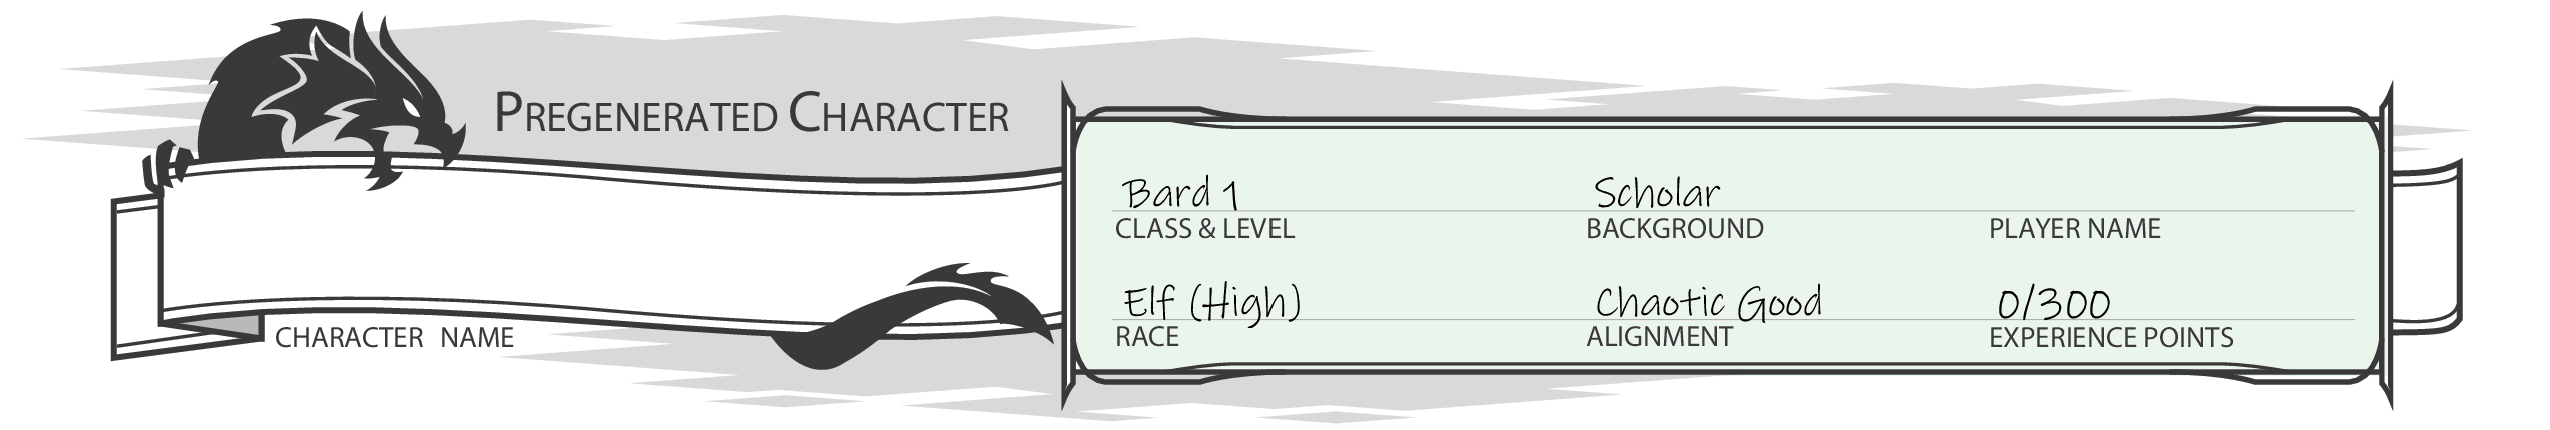
\includegraphics[width=\textwidth]{splash.png}};

  \colorlet{splashgray}{white!85.765!black}

  \begingroup\sffamily

  \newcommand\namestrut{\vrule width 0pt depth 1pt\relax}

  \path ($(splash.south west)+(88mm,18.75mm)$) coordinate  (class field sw);
  \path ($(splash.south west)+(88mm,9.7mm)$) coordinate  (race field sw);
  \path ($(splash.south west)+(48mm,16mm)$) coordinate  (charname center);
  \path ($(splash.south west)+(40mm,24mm)$) coordinate  (pregen left);
 

  \ifDNDfalse{PREGENERATED}%
    {\node [fill=splashgray,width=42mm,height=5mm,anchor=south west,at=(pregen left)] {};}
    {}


  \node [fill=splashfield,width=97mm,height=6mm,anchor=south west,at=(class field sw)] {};
  \node [fill=splashfield,width=97mm,height=6mm,anchor=south west,at=(race field sw)] {};

  \path (class field sw) +(0mm,0.6mm) coordinate (class sw);
  \path (race field sw) +(0mm,0.6mm) coordinate (race sw);

  \writesplash[at=(class sw)]{34mm}{CLASS + LEVEL}
  \writesplash[right of base=1mm of CLASS + LEVEL]{28mm}{BACKGROUND}
  \writesplash[right of base=1mm of BACKGROUND]{34mm}{PLAYER NAME}

  \writesplash[at=(race sw)]{34mm}{RACE}
  \writesplash[right of base=1mm of RACE]{34mm}{ALIGNMENT}
  \writesplash[right of base=1mm of ALIGNMENT]{34mm}{EXPERIENCE POINTS}

  \ifDNDdefined{CHARACTER NAME}
{\node[at=(charname center),font={\rmfamily\LARGE\itshape},anchor=center]
      {\getDND{CHARACTER NAME}\ifDNDnonempty{AGE}{ \Large (\getDND{AGE})}{}}
      ;
    }
    {}

  \path (splash.south |- bottom right) coordinate (bottom center);

  %%% central column: hit-point thing, equipment, attacks fill

\Large

      \node (hpbackground) 
        [stub rectangle,yseparated,fill=hit points background,below=of splash,width=\colwidth, minimum height=87mm] 
       { };

\begin{scope}[node distance=\mynodedistance]

      \node (initiative)
            [initiative,below=of hpbackground.north] 
         {\nodepart{label}\footnotesize INITIATIVE\nodepart{ctext}\getDND*{INITIATIVE}}
         ;

       \node (ac) [initiative,shield,inner shield,draw,ultra thick,left=of initiative,width=12mm,
                   font=\Large,
            ]
      {\getDND*{ARMOR CLASS}}
      ;

      \node [above=3pt of ac.south] {\tinystacklabel{ARMOR}{CLASS}};

      \node (speed) [initiative,right=of initiative]
         {\nodepart{ctext}\getDND*{SPEED}\nodepart{label}SPEED}
         ;

%      \draw [thick,black,fill=yellow] (speed.labeltop) circle [radius=5pt];

      \node [dnd max hp2,below=of initiative,width=\hpwidth] 
         (maxhp)
         {\nodepart{label}CURRENT HIT POINTS}
         ;
      \node [below=of maxhp.north,font=\scriptsize] {%
         \hbox to \hpwidth{%
             ~~~Maximum Hit Points~~\rlap{\raisebox{4pt}{\smash{\normalsize~~~\getDND*{MAX HP}}}}%
               \hrulefill~~~}}
       ;

      \node[dnd max hp2,below=of maxhp,minimum height=20mm,width=\hpwidth]
        (temphp)
        {\nodepart{label}TEMPORARY HIT POINTS}
        ;



      \node (hitdice)
             [dnd hit dice,below left corner=of temphp] 
         {\nodepart{label}HIT DICE\nodepart{ctext}
            \vrule height 8mm width 0pt\Large\getDND*{HIT DICE}}
         ;

     \ifDNDdefined{LEVEL}{
         \node [at=(hitdice.north),anchor=north] 
              {\expandafter\stackslots\expandafter{\rawgetDND{LEVEL}+1}};
     }{}

      \node (death saves)
            [dnd hit dice,below right corner=of temphp,font=\small] 
         { \nodepart{label}DEATH SAVES\nodepart{ctext}
            \tiny\begin{tabular}{@{}r@{\hskip1pt}l@{}}
            \raisebox{1pt}{SUCCESSES}&\slotsliteral3\\[2pt]
            \vrule width 0pt depth 5pt\raisebox{1pt}{FAILURES}&\slotsliteral3\\
            \end{tabular}
          }
         ;


%\node [draw,above=of initiative] % {\slotsliteral7};
%              {\expandafter\stackslots\expandafter{\rawgetDND{LEVEL}+1}};


\end{scope}

  \endgroup


\makeatletter
\renewcommand\attackkeys[1]{%
  \gdef\@attackname{}%
  \gdef\@attackattack{}%
  \gdef\@attackdamage{}%
  \gdef\@attacktype{}%
  \gdef\@attackrange{}%
  \gdef\@attackammo{}%
  \pgfkeys{/attacks/.cd, #1}%
  \small \@attackname&\@attackattack&\@attackdamage\ \small\@attacktype\\
}
\makeatother


\newdimen\attacksInnerSep
\attacksInnerSep=4pt



\node[columnbox,anchor=north east] (motivation) at (splash.east |- hpbackground.north)
   {\nodepart{label}DESCRIPTION \&\ PERSONALITY
    \nodepart{text}%
    \newcommand\hangpar{\hangindent=1em \hangafter=1 \par}%
    \smallskip
    Motivation:\\
    \getDND*{MOTIVATION}
    \hangpar
    \bigskip
    \ifDNDnonempty{SUGGESTED MOTIVATIONS}{%
       Suggested Motivations:\\ \getDND{SUGGESTED MOTIVATIONS} \hangpar
       \bigskip
    }{}
    \ifDNDnonempty{SUGGESTED NAMES}{%
       Suggested Names:\\ \getDND{SUGGESTED NAMES} \hangpar
       \bigskip
    }{}
    \hbox{}
   }
;



\newenvironment{itemize spells}
  {\clubpenalty=10000
   \widowpenalty=10000
   \begin{itemize}[topsep=0pt,itemsep=0pt,leftmargin=6pt,parsep=0pt,labelsep=2pt]
  }%
  {\end{itemize}}

\node (features top) [below=of motivation] {};
\setdeltay\sectionheight{features top}{bottom right}


\ifDNDdefined{FEATURES}{%
  %%% XXX drops below bottom right
  \node (features) [columnbox,height=\sectionheight,fill=features,below=of motivation]  {
    \nodepart{label}{FEATURES \&\ TRAITS}\nodepart{text}%
    \long\def\described#1#2{\strut\emph{#1:} #2\par\smallskip}%
    \getDND{FEATURES}

    \ifDNDnonempty{MAGIC}{%
      \smallskip
      \footnotesize
      \newcommand\spellslevellabel[2]{%
        \ifnum#1=0
           Cantrips: You can cast these spells as often as you like using 1~action.
        \else
           \end{itemize spells}
           Level~#1 spells: Cast these spells in any combination%
           \ifnum#2>0\relax
              \ #2~times per long rest.
           \else
              .
           \fi
          Casting is 1~action unless noted.
        \fi
        \begin{itemize spells}
      }
      \long\def\described#1#2{\item #1: #2}%
      \getDND{MAGIC}
      \end{itemize spells}
    }{}
  }
  ;
}{}

\setnodewidth\sectionwidth[statbox]
\node (stats background) 
      [stub rectangle,stub radius=6pt,fill=stats,width=\sectionwidth+4mm,height=163mm,anchor=north west]
      at (splash.west |- hpbackground.north)
 { };

\path (stats background.north west) ++(2mm,-2.2mm) coordinate (first stat);
\renewcommand\nextstatloc{anchor=north west,at=(first stat)}



\dndstat{STRENGTH}{STR}
\dndstat{DEXTERITY}{DEX}
\dndstat{CONSTITUTION}{CON}
\dndstat{INTELLIGENCE}{INT}
\dndstat{WISDOM}{WIS}
\dndstat{CHARISMA}{CHA}

\node (dummy left column) [columnbox,shape=rectangle,draw=none,anchor=west] 
   at (stats background.west)
   {}
   ;

\path (dummy left column.east |- stats background.north)
      ++(0,-1mm) % don't let box stick out too much
       coordinate (inspo right)
    ; 

\setdeltax\sectionwidth{inspo right}{stats background.east}
\advance\sectionwidth by -\mynodedistance

\node (inspiration)
      [fill=white,draw,line width=1.2pt,decorated stub rectangle,width=\sectionwidth-5mm,
      height=8mm,
      anchor=north east, at=(inspo right)
      ]
   {}
   ;
\node [anchor=west,proficiencies,fill=white,stub rectangle,
       width=10mm,height=10mm,line width=1.5pt,draw]
       at ($(inspiration.west)+(-5mm,0mm)$)
      (inspo box)
      {};

\node  [fill=none,stub rectangle,
       width=10mm,stub radius=2.5mm,height=10mm,line width=0.5pt,scale=0.85,draw]
       at (inspo box)
      {};

% center the name in the visible space
\setdeltax\tmpwidth{inspiration.east}{inspo box.east}

\path (inspo box.east) ++(0.5\tmpwidth,0) node
      {\small\textsf{INSPIRATION}};


\node[columnbox,text width=,width=\sectionwidth,% width=38.002mm,
      fill=white,below right corner=3.5mm of inspiration,align=center,
      height=35mm,
    ]
    (saving throws)
    {\nodepart{label}SAVING THROWS\nodepart{text}%
     \vspace*{3pt}
     \renewcommand\arraystretch{1.15}%
     \tabcolsep=2pt
     \scshape
     \begin{tabular}{@{}rll@{}}
      \dndsavingthrow{STR}&\normalsize Strength    &\savemark{STR}\\
      \dndsavingthrow{DEX}&\normalsize Dexterity   &\savemark{DEX}\\
      \dndsavingthrow{CON}&\normalsize Constitution&\savemark{CON}\\
      \dndsavingthrow{INT}&\normalsize Intelligence&\savemark{INT}\\
      \dndsavingthrow{WIS}&\normalsize Wisdom      &\savemark{WIS}\\
      \dndsavingthrow{CHA}&\normalsize Charisma    &\savemark{CHA}\\
    \end{tabular}}
  ;
\node (proficiency bonus)
      [proficiencies,decorated stub rectangle,width=\sectionwidth-2mm,height=8mm,
       below right corner=4mm of saving throws]
   {\hbox to 0pt{\hss\hspace*{6.2mm}\scriptsize\textsf{PROFICIENCY BONUS}\hss}}
   ;
\node (proficiency circle) [anchor=west,proficiencies,circle,inner circle,
       width=10mm,height=10mm,line width=1.5pt,draw]
       at ($(proficiency bonus.west)+(-2mm,0mm)$)
      {\large\textsf{+\arabic{proficiency bonus}}};


  \setdeltay\sectionheight{proficiency bonus.south}{stats background.south}
  \advance\sectionheight by -3mm
  \node (proficiencies) [columnbox,text width=\sectionwidth-2\textmargin,fill=proficiencies,height=\sectionheight,
        anchor=south east,at=(stats background.south -| saving throws.east)]
   {\nodepart{label}PROFICIENCIES\nodepart{text}%
    \ifDNDdefined{PROFICIENCIES}{%
     \long\def\split#1\profskip#2\nil{%
       \def\profbefore{#1}% before part
       \def\profafter{#2}%  after part (empty if no \profskip in input)
     }%
\begin{proflist}
     \expandafter\expandafter\expandafter\expandafter\expandafter\expandafter\expandafter\split\rawgetDND{PROFICIENCIES}\profskip\nil
     \profbefore
     \expandafter\gdef\expandafter\otherproficiencies\expandafter{\profafter}%
%\item Long proficiency that really will not fit on one line
\end{proflist}
   }{%
     (None specified)
   }%
   }
   ;

%\draw [red,fill=green] (proficiencies.north east) circle [radius=3.5pt];
%\draw [red,fill=blue!10!white] (proficiencies.south west) circle [radius=3.5pt];
%\draw [red,fill=yellow] (proficiencies.text) circle [radius=3.5pt];
%\draw [red,fill=red!20!white] (proficiencies.label) circle [radius=3.5pt];
%
%\draw [fill=red] (prof bot fit) circle [radius=5pt];
%\draw [fill=red] (prof top fit) rectangle ++(5pt,5pt);

%\node (motivation) [below=of proficiencies] 
%  {\parbox{36mm}{\Large\centering\textit{\getDND*{MOTIVATION}}}}
%  ;


\ifDNDdefined{EQUIPMENT}{%

  \node (equipment) [columnbox,decorated labeled clipped rectangle,fill=equipment,
                     minimum height=124pt, % make enough room for coins
                     anchor=south,at=(bottom center |- features.south)]
   {%
     \nodepart{label}EQUIPMENT\nodepart{text}
     \medskip
     \noindent
     \hspace*{21mm}%
     \begin{minipage}{\hsize-21mm}
     \small
      \begin{eqlist}%
     \ifDNDnonempty{EQUIPMENT}{}{%
       \item \noindent\vrule width 0pt height 0pt depth 8\baselineskip (Placeholder: Equipment will go here.)
     }%
     \useDNDfont{EQUIPMENT}%
     \getDND{EQUIPMENT}
    \end{eqlist}%
     \end{minipage}%
   }
  ;
}
{\node (equipment) [at=(bottom center)] {};
}

\path (equipment.south west) +(5mm,40mm) coordinate (coin top left);


\coin{cp}{Cu}{\color{grayed out}\getDND*{CP}}
\coin{sp}{Ag}{\color{grayed out}\getDND*{SP}}
\coin{gp}{Au}{\color{grayed out}\getDND*{GP}}
\coin{pp}{Pt}{\color{grayed out}\getDND*{PP}}
  
%%%%%% attacks

\newenvironment{attackstab*}
  {\renewcommand\arraystretch{1.3}%
   \def\notesheader{\multicolumn3{@{}l}{\vrule width 0pt height 18pt\small\textsf{\textit{NOTES}}}\\}%
   \renewcommand\attacknote[2]{\small ##1:&\multicolumn2{@{}l@{ }}{\small##2}\\}%
   \tabcolsep=0.5\tabcolsep
   \normalsize
   \let\dndkeys=\attackkeys
   \noindent
   \hspace*{\attacksInnerSep}%   
   \begin{tabular*}{\hsize-2\attacksInnerSep}{@{}lll@{}}
   \textsf{\footnotesize NAME}&
   \textsf{\scriptsize \llap{ATK BO}NUS}&
   \textsf{\scriptsize DAMAGE/TYPE}\\
   \midrule
  }
  {\end{tabular*}\hspace*{\attacksInnerSep}\par}

\node (attacks bottom) [above=of equipment] {};

\setdeltay\sectionheight{hpbackground.south}{attacks bottom.north}


  \node (attacks) [columnbox,fill=attacks,height=\sectionheight,
                   below=of hpbackground,
%at={(0,0)},
%   anchor=north,at=(hpbackground.south),
]
   {
    \nodepart{label}ATTACKS\nodepart{text}%
    \centering
    \useDNDfont*{ATTACKS}
    \begin{attackstab*}
    \getDND{ATTACKS}
    \end{attackstab*}

    \medskip

    \begin{minipage}{\hsize-2\attacksInnerSep}
    \small
    \def\notesheader{}
    \renewcommand\attacknote[2]{}
    \useDNDfont*{ATTACKS}
    \DNDranges
    \end{minipage}
    \vfill
   }
;

%\draw (hpbackground.south) [red] circle [radius=3pt];
%\draw (equipment.north) [red] circle [radius=3pt];
%
%\draw (attacks.south) [blue] circle [radius=3pt];
%\draw (attacks.north) [blue] circle [radius=3pt];
%
%\path [fill=white] (attacks.south) circle [radius=0.5pt];


\node (motivations) [above=4.45mm of BACKGROUND.north] 
  {\Large\textit{\getDND*{MOTIVATION}}}
  ;


%%% left-hand column

\node (passive perception)
      [decorated stub rectangle,width=\colwidth-8mm,height=8mm,
       line width=1.2pt,draw,
       below right corner=of proficiencies]
   {\hbox to 0pt{\hss\footnotesize\textsf{PASSIVE WISDOM (PERCEPTION)}\hss}}
   ;

\node (perception box)
      [anchor=east,chamfered rectangle,chamfered rectangle angle=60,fill=white,
       width=10mm,height=9mm,line width=2.0pt,draw]
       at ($(passive perception.west)+(+4mm,0mm)$)
      {\ifDNDnonempty{PASSIVE PERCEPTION}
         {\large\textsf{\signed{\rawgetDND{PASSIVE PERCEPTION}}}}
         {?}
      }
      ;
% because angles, no way this geometry can look good:
% need different scales in x and y to get proper inset
% (hey) node [chamfered rectangle,chamfered rectangle angle=60,width=10mm,height=9mm,line width=0.5pt,blue,scale=0.8,draw,fill=none]  {}

\node [fill=none,draw,line width=0.5pt,chamfered rectangle,
       chamfered rectangle angle=60,width=9.6mm,height=7.4mm] 
      at (perception box)
      {}
      ;


\node (other proficiencies top) [below=of passive perception] { };

\setdeltay\sectionheight{other proficiencies top}{bottom left}

\node [anchor=south west,columnbox,minimum height=\sectionheight,
      ]
   (other proficiencies)
   at (stats background.west |- features.south)
  {\nodepart{label}\scriptsize WEAPON, ARMOR, \&\ LANGUAGE PROFICIENCIES
   \nodepart{text}%
   \multicolsep=0pt
    \begin{multicols}{2}
    \begin{proflist}
    \itemsep=1pt
    \otherproficiencies
    \end{proflist}
    \end{multicols}
  }
  ;

\end{charsheet}

% Equipment Weight Summary Page
\clearpage

\begin{charsheet}

\sffamily


% Define colors for capacity boxes
\colorlet{carrying}{white}
\colorlet{encumbered}{proficiencies}  % Use existing yellow from charsheet.sty
\colorlet{heavilyencumbered}{magic}   % Use existing red from charsheet.sty
\colorlet{unencumbered}{equipment}

% Define height per tenth of stone for equipment slots
\newdimen\tenthstoneheight
\tenthstoneheight=8pt

% Calculate carrying capacity thresholds (in tenths of stones)
\newcounter{carryingCapacity}
\newcounter{encumberedThreshold}
\newcounter{heavilyEncumberedThreshold}

\ifDNDnonempty{STR}{%
  % Carrying capacity = STR score in stones (convert to tenths)
  \setcounter{carryingCapacity}{\numexpr\rawgetDND{STR} * 10\relax}
  
  % Encumbered = 1/3 of carrying capacity, rounded down
  \setcounter{encumberedThreshold}{\numexpr\rawgetDND{STR} * 10 / 3\relax}
  
  % Heavily encumbered = 2/3 of carrying capacity, rounded down  
  \setcounter{heavilyEncumberedThreshold}{\numexpr\rawgetDND{STR} * 20 / 3\relax}
}{%
  % No STR defined - leave counters at zero
}

\node (banner) [below=of top]
      {\LARGE{\textsf{\textbf{Equipment and Encumbrance by Stones%
        \ifDNDnonempty{CHARACTER NAME}{ (\getDND{CHARACTER NAME})}{}}}}};

% Calculate total weight (in tenths of stones)
\newcounter{significantWeight}
\withitemweight{\setcounter{significantWeight}}{HEAVY WEAPONS}
\withitemweight{\addtocounter{significantWeight}}{NORMAL WEAPONS}
\withitemweight{\addtocounter{significantWeight}}{SHIELDS}
\withitemweight{\addtocounter{significantWeight}}{HEAVY ARMOR}
\withitemweight{\addtocounter{significantWeight}}{MEDIUM ARMOR}
\withitemweight{\addtocounter{significantWeight}}{LIGHT ARMOR}
\withitemweight{\addtocounter{significantWeight}}{HEAVY ITEMS}

\newcounter{remainingCapacity}
\ifDNDnonempty{STR}{%
  % Remaining = carrying capacity - significant weight (in tenths of stones)
  \setcounter{remainingCapacity}{\numexpr\rawgetDND{STR} * 10 - \value{significantWeight}\relax}
  % Convert to stones and multiply by 5 for line count
  \setcounter{remainingCapacity}{\numexpr\value{remainingCapacity} * 5 / 10\relax}
}{%
  \setcounter{remainingCapacity}{0}
}

% Equipment slots box on the left with three-color backgrounds
% First calculate positions for color transitions in terms of \tenthstoneheight
\newcounter{greenLines}
\newcounter{yellowLines}  
\newcounter{redLines}

\ifDNDnonempty{STR}{%
  % Calculate how many lines each color region should have
  % Total lines = 5 * remaining capacity (in stones)
  % Use PGF arithmetic for truncation instead of \numexpr rounding
  % \pgfmathtruncatemacro truncates toward zero, giving us floor division for positive numbers

  %% use at most 43 slots
  \pgfmathtruncatemacro{\greenlines}{
    min(43, floor(((\value{encumberedThreshold}-\value{significantWeight})*5)/10))
  }
  % Clamp yellow to what's left
  \pgfmathtruncatemacro{\yellowlines}{
    max(0, min(43-\greenlines, floor(((\value{heavilyEncumberedThreshold}-\value{significantWeight})*5)/10)))
  }
  % Clamp red to what's left after green+yellow
  \pgfmathtruncatemacro{\redlines}{
    max(0, min(43-\greenlines-\yellowlines, ((\value{carryingCapacity}-\value{heavilyEncumberedThreshold})*5)/10))
  }
  \setcounter{greenLines}{\greenlines}
  \setcounter{yellowLines}{\yellowlines}
  \setcounter{redLines}{\redlines}
}{%
  \setcounter{greenLines}{0}%
  \setcounter{yellowLines}{0}%
  \setcounter{redLines}{0}%
}

% Calculate heights for each color region
\newdimen\greenheight
\newdimen\yellowheight
\newdimen\redheight

\greenheight=\numexpr2*\value{greenLines}\relax\tenthstoneheight
\yellowheight=\numexpr2*\value{yellowLines}\relax\tenthstoneheight  
\redheight=\numexpr2*\value{redLines}\relax\tenthstoneheight


\path (top left) 
 ++(0, -13mm)
  node (slotstitle)
    [slotblock,anchor=north west,fill=blue!10!white,minimum height=28pt] 
  {\Large\textbf{Slotted Items}}
  ;

% Three capacity boxes centered below top
\path (slotstitle.north east) ++(20pt,0)
 node (carrying) [dndencumbrance,fill=carrying,anchor=north west]
  {\nodepart{label}CARRYING CAPACITY\nodepart{ctext}
   \Large\ifDNDnonempty{STR}{$\mathbf{\leq\renderstones{\arabic{carryingCapacity}}}$}{}
  };

\node (encumbered) [dndencumbrance,fill=encumbered,right=5mm of carrying] 
  {\nodepart{label}ENCUMBERED\nodepart{ctext}
   \Large\ifDNDnonempty{STR}{$\mathbf{\geq\renderstones{\arabic{encumberedThreshold}}}$}{emptyb
  STR?}};

\node (heavily) [dndencumbrance,fill=heavilyencumbered,right=5mm of encumbered]
  {\nodepart{label}HEAVILY ENCUMBERED\nodepart{ctext}
   \Large\ifDNDnonempty{STR}{$\mathbf{\geq \renderstones{\arabic{heavilyEncumberedThreshold}}}$}{}
  };


\node (e warning) [below=of encumbered] {\small(Speed drops by 10~ft)};
\node (h warning) [below=of heavily,inner sep=2pt] {%
  \hspace*{3mm}%
  \begin{minipage}{40mm}\raggedright
   \small
   (Speed drops by 20~ft;
   Disadvantage on ability checks, saving throws, and attack rolls that use \scrm{str}, \scrm{dex}, or \scrm{con}.)
   \end{minipage}}
  ;


\path (slotstitle) coordinate (slotsbottom);

\ifdim\greenheight>0pt

  \node (slotgreen) [slotblock,fill=unencumbered,anchor=north west,
                     minimum height=\greenheight]
    at (slotstitle.south west) {} ;

  \path (slotgreen.south west) coordinate (slotsbottom);


  \ifdim\yellowheight>0pt

     \node (slotyellow) [slotblock,fill=encumbered,anchor=north west,
                        minimum height=\yellowheight]
       at (slotgreen.south west) {} ;

     \path (slotyellow.south west) coordinate (slotsbottom);


     \ifdim\redheight>0pt

        \node (slotred) [slotblock,fill=heavilyencumbered,anchor=north west,
                           minimum height=\redheight]
          at (slotyellow.south west) {} ;

        \path (slotred.south west) coordinate (slotsbottom);



     \fi
  \fi
\fi

\foreach \deltay in {1,2,...,\numexpr\value{greenLines}+\value{yellowLines}+\value{redLines}\relax} {
  \draw (slotstitle.south west)
    ++(8pt,-\deltay*2*\tenthstoneheight)
    -- ++(\slotblockwidth-2\textmargin,0)
   ;
}

\path (slotstitle.south west) ++(5pt,2pt) coordinate (lastslot);

\begingroup
  \newcommand\DNDitem[2]{%
     \path (lastslot)
       ++(0,-2\tenthstoneheight)
       node [anchor=base west] (thisslot) {\color{grayed out}#1};
     \path (thisslot.base west) coordinate (lastslot);
  }
  \doDNDitems{LIGHT WEAPONS}
  \doDNDitems{SLOTTED ITEMS}
\endgroup

\path (slotsbottom) ++(1pt,2pt) coordinate (decor ll)
      (slotstitle.north east) ++(-1pt,-2pt) coordinate (decor ur)
  ;

\node [draw,decorated stub rectangle,thick,
    stub radius=\dndStubRadius,
    line width=1.2pt,
        fit=(decor ll) (decor ur),
      ]
  (slots decoration)
  {};


%
%  \foreach \thing in {{fish},{fowl},{fury}} {
%     \node [anchor=north] at (lastslot.south) (thisslot) {\thing};
%     \path (thisslot.south) coordinate (lastslot);
%  }
%


%%%%    \node [dndbox,slotblock,below=5mm of heavy equipment,fill=equipment,inner sep=15pt] 
%%%%       (worn items)
%%%%    {
%%%%      \def\arraystretch{1.32}%
%%%%    %  \newcommand{\DNDitem}[2]{#1&$\mathbf{\renderstones{#2}}$&\stonesplural{#2}\crcr}%
%%%%      \newcommand{\DNDitem}[2]{#1\crcr}%
%%%%      \begin{tabular}{l}
%%%%      \multicolumn1{c}{\bigstrut \Large \textbf{Worn Items}}\\[5pt]
%%%%      % Local definition of \DNDitem for display
%%%%      % Display all significant equipment items
%%%%      \doDNDitems{WORN ITEMS}%
%%%%    %  Z\crcr
%%%%    %  \midrule
%%%%    %  \doDNDitems{SLOTTED ITEMS}%
%%%%    %  Total&$\mathbf{\renderstones{\value{significantWeight}}}$&\stonesplural{\value{significantWeight}}\\
%%%%      \end{tabular}%
%%%%    };

%\path (heavily.east |- h warning.south) coordinate (h warning r);

\node [dndbox,slotblock,anchor=south east,at=(heavily.east |- slots decoration.south),
       fill=equipment,minimum height= 74\tenthstoneheight]
  (small items)
  { }
;

\node [below top=5mm of small items,minimum width=\slotblockwidth] (smalltitle) {\Large\textbf{Small Items}};

\foreach \deltay in {1,2,...,34} {
  \draw (smalltitle.south west)
    ++(12pt,-\deltay*2*\tenthstoneheight)
    -- ++(\slotblockwidth-24pt,0)
   ;
}

\begingroup
  \path (smalltitle.south west) ++(9pt, 2pt) coordinate (lastslot);
  \newcommand\DNDitem[2]{%
     \path (lastslot)
       ++(0,-2\tenthstoneheight)
       node [anchor=base west] (thisslot) {\color{black!30!white}#1};
     \path (thisslot.base west) coordinate (lastslot);
  }
  \doDNDitems{SMALL ITEMS}
\endgroup


% Equipment weight breakdown table
\node [dndbox,anchor=north west,at=(carrying.west |- small items.north),fill=equipment,inner sep=15pt] 
   (heavy equipment)
{
  \def\arraystretch{1.32}%
  \newcommand{\DNDitem}[2]{#1&$\mathbf{\renderstones{#2}}$&\stonesplural{#2}\\}%
  \begin{tabular}{lr@{~}l}
  \multicolumn3{c}{\bigstrut \Large \textbf{Heavy Equipment}}\\[5pt]
  \doDNDitems{HEAVY WEAPONS}%
  \doDNDitems{NORMAL WEAPONS}%
  \doDNDitems{SHIELDS}%
  \doDNDitems{HEAVY ARMOR}%
  \doDNDitems{MEDIUM ARMOR}%
  \doDNDitems{LIGHT ARMOR}%
  \doDNDitems{HEAVY ITEMS}%
  \midrule
  Total&$\mathbf{\renderstones{\value{significantWeight}}}$&\stonesplural{\value{significantWeight}}\\
  \end{tabular}%
};




\node [slotblock,anchor=south west,inner sep=0pt]
  at (slots decoration.south -| heavy equipment.west)
  {\Large\begin{tabular}{@{}l@{ = }l@{}}
   1 Slot &Bundle of up to 20\\
   \multicolumn1{@{}l@{}}{}&identical items, \emph{or}\\[3pt]
   \multicolumn1{@{}l@{}}{}&150~coins, \emph{or}\\[3pt]
   \multicolumn1{@{}l@{}}{}&1 stowed weapon\\[8pt]
   5 Slots&1 Stone\\
  \end{tabular}}
;
   


  
\end{charsheet}

\ifDNDfalse{VALIDATION ERRORS}{}
{
\section{Validation errors}
\begin{itemize}
\getDND{VALIDATION ERRORS}
\end{itemize}
}

\end{document}
